\subsection{Plan Overview}
The four tiers that constitute the System (Client Application, Web Server, Application Server, and Data Manager) represent distinct functional layers that can be implemented primarily in parallel. By defining the interfaces early in the process such as the AccountServiceI, TripServiceI, and PathServiceI exposed by the Web Server development teams can work simultaneously on the client-side presentation and the server-side logic, integrating them continuously.

\vspace{10pt}
\noindent
The Application Server layer encapsulates the core business logic and presents internal dependencies that require a more structured approach. For this central component, a bottom-up approach will be adopted. This strategy dictates starting with the implementation of independent and low-level modules before moving to those that orchestrate complex workflows.

\vspace{10pt}
\noindent
The following diagram details the dependencies between the various components of the Application Server, including the relationships with the proxy component responsible for external data retrieval. In this representation, a hierarchical convention applies: if a component depicts a dependency on another component, it implies that all its internal sub-components share this dependency. Conversely, if a dependency is exclusive to a specific sub-component, a direct link is established solely to that element.

\begin{figure}[H]
    \centering
    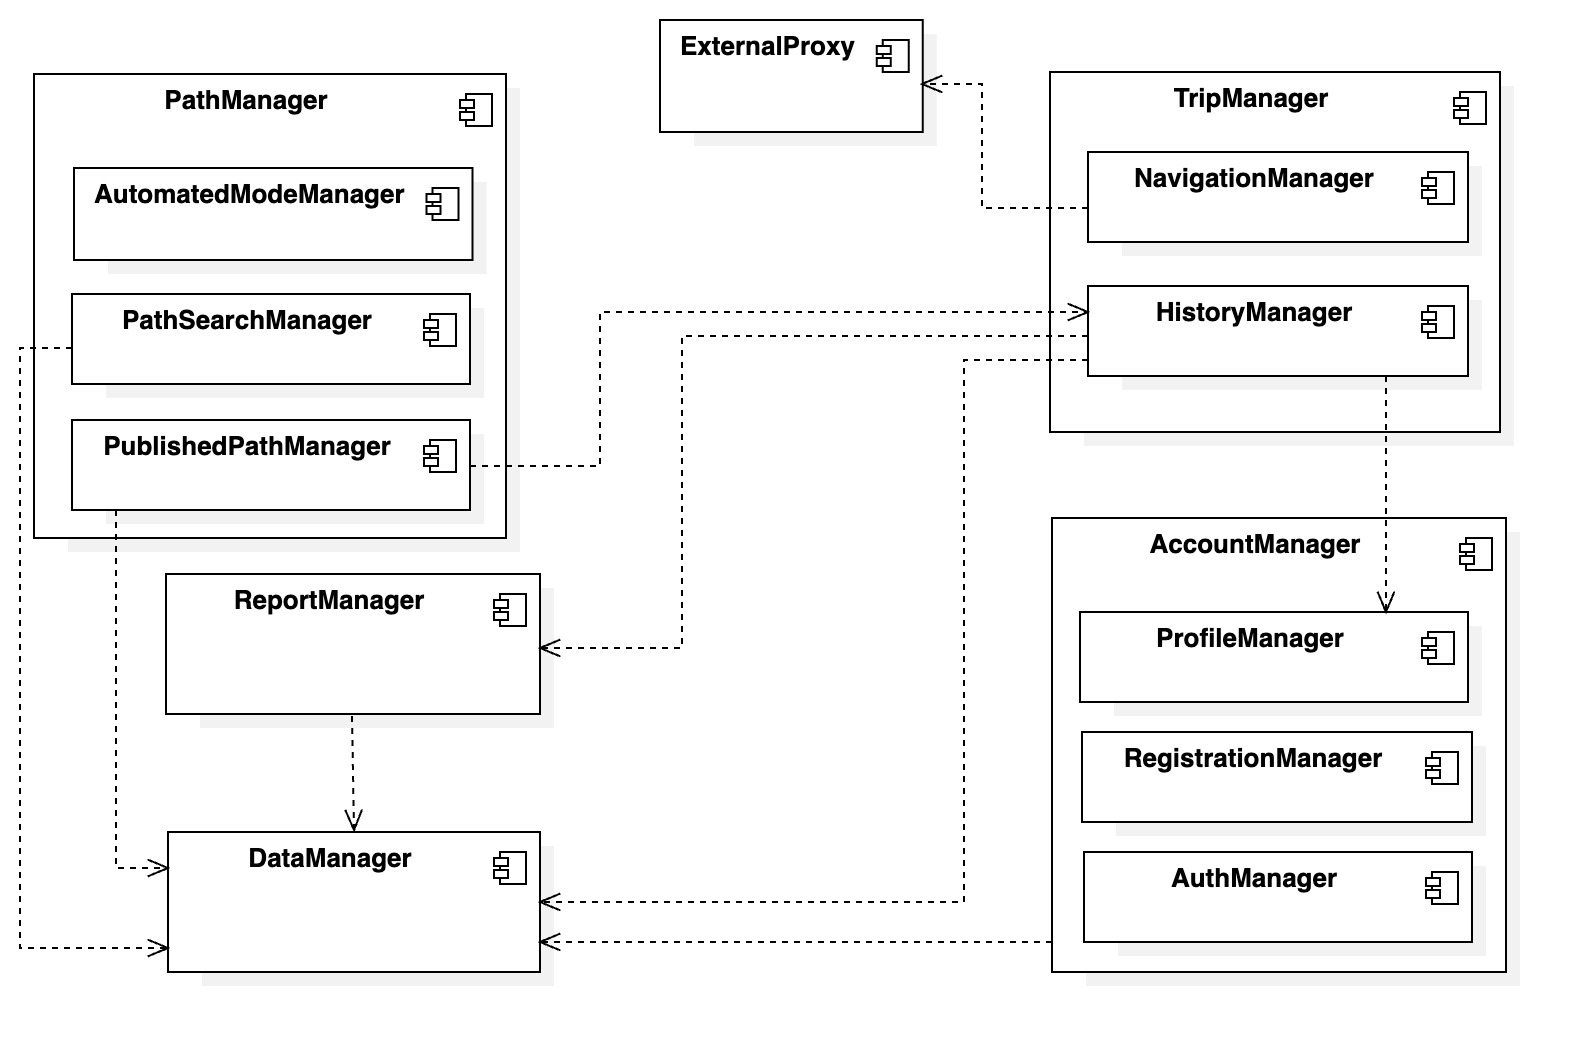
\includegraphics[width=0.9\linewidth]{DD//Images//Implementation/DependenciesDiagram.jpg}
    \caption{Dependencies Diagram}
    \label{fig:placeholder}
\end{figure}

\newpage
\subsection{Implementation Plan}
The following plan focuses strictly on the Application Server components and the External Proxy, where the dependency chain dictates a sequential implementation order.

\begin{enumerate}
    %1 DataManager
    \item \textbf{DataManager:} This is the first module to be implemented. Indeed, all the other components of the Application Server rely on it to communicate with the Database. Therefore, it is a module of crucial importance but characterized by a low level of functional complexity as it primarily implements the queries and CRUD operations.
    
    %2 ExternalProxy
    \item \textbf{ExternalProxy:} This component is developed in parallel with or immediately after the DataManager. It is responsible for abstracting the communication with external systems, specifically the WeatherService. Its early implementation is essential to provide the necessary weather data of the trips (managed by TripManager).

    %3 AccountManager
    \item \textbf{AccountManager}: The implementation of this module follows. It comprises the AuthManager, RegistrationManager, and ProfileManager. Its development is prioritized because it establishes the user context required by the subsequent components. Specifically, the ProfileManager exposes the interfaces necessary to manage user data.

    %4 ReportManager
    \item \textbf{ReportManager} This component acts independently of the user logic and can be implemented at this stage. It manages the reports and implements a specific aggregation logic to merge multiple reports generated by different users for the same path within the same day. It interacts directly with the DataManager for persistence. Its completion is a prerequisite for the TripManager, as the reporting logic is triggered by completed trips.

    %5 TripManager
    \item \textbf{TripManager}: This component is implemented at this stage. It contains the NavigationManager and the HistoryManager. Its development relies on the completion of both the AccountManager and the ReportManager. The HistoryManager explicitly depends on the ProfileManager to update user statistics upon trip completion, and on ReportManager to submit user-generated reports. The NavigationManager depends on the ExternalProxy for the weather service API calls.

    %6 PathManager
    \item \textbf{PathManager}: This is the final module to be implemented. It contains the PathSearchManager, AutomatedModeManager, and PublishedPathManager.
    This component is placed last in the sequence due to a specific functional dependency: the PublishedPathManager requires access to the HistoryManager (part of the TripManager) to save the trip details into the user's history once an automated path acquisition is concluded.
\end{enumerate}

\newpage
\subsection{Component Integration and Testing}
This section describes the integration plan for the system components. Each component must first undergo Unit Testing in isolation. The integration process then occurs incrementally following a Bottom-Up approach: as soon as a component at a lower dependency level is stable, it is integrated with the components of the upper level.
\vspace{10pt}

\noindent
To facilitate this process before the complete system is available, we will utilize Test Drivers: software modules used to invoke the component under test, simulating the requests that would normally come from the Web Server or other managers. The integration sequence is organized into four logical stages:
\vspace{10pt}

\noindent
\textbf{Stage 1: Data Persistence and External Services}
\vspace{2pt}

\noindent
In the first stage, we focus on the integration of the DataManager and the ExternalProxy, which act as the foundational layer of the Application Server. Since these components interact directly with the Database and external services respectively, their stability is a prerequisite for the entire system. Because the higher-level managers (such as the AccountManager or TripManager) are not yet developed at this stage, we utilize Test Drivers to simulate the invocation of these components:

\begin{itemize}
    \item A Persistence Driver is developed to simulate the queries that will eventually be performed by the business logic, verifying the DataManager's ability to execute CRUD operations correctly.
    \item A Proxy Driver is created to simulate requests for weather data, ensuring that the ExternalProxy correctly interfaces with the WeatherService API and parses its response.
\end{itemize}

\noindent
The following diagram illustrates this initial integration step, showing the drivers stimulating the base components in isolation.

\begin{figure}[H]
    \centering
    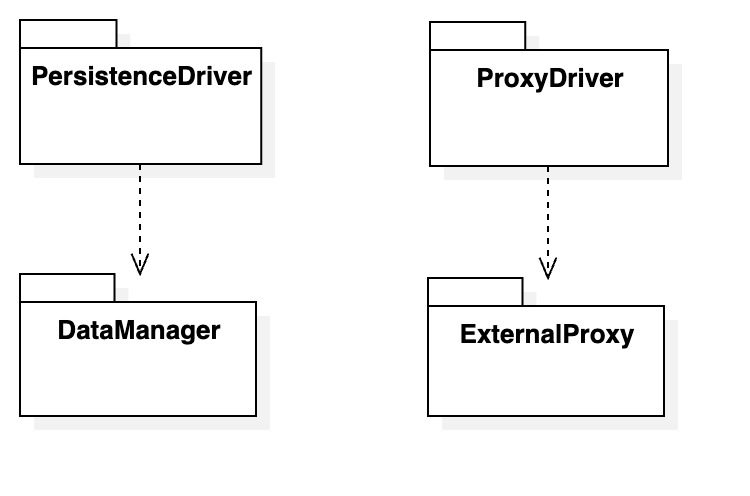
\includegraphics[width=0.6\linewidth]{DD//Images//Implementation/Stage1.jpg}
    \caption{Stage 1}
    \label{fig:placeholder}
\end{figure}

\newpage
\noindent
\textbf{Stage 2: Independent Business Managers}
\vspace{2pt}

\noindent
The second stage involves the integration of the AccountManager and the ReportManager. These components are built upon the persistence layer validated in the previous stage. Since these managers are functionally independent of each other but rely on the DataManager for data storage and retrieval, they are integrated in parallel:

\begin{itemize}
    \item The AccountManager is connected to the DataManager to verify that user registration, authentication, and profile updates are correctly persisted in the database.
    \item The ReportManager is integrated with the DataManager to ensure that infrastructure reports are correctly stored and that the aggregation (merging) logic successfully retrieves existing reports from the database.
\end{itemize}
\vspace{3pt}

\noindent
To simulate the requests that would normally originate from the Web Server or the TripManager, specific Drivers are employed to invoke the methods exposed by these components.

\begin{figure}[H]
    \centering
    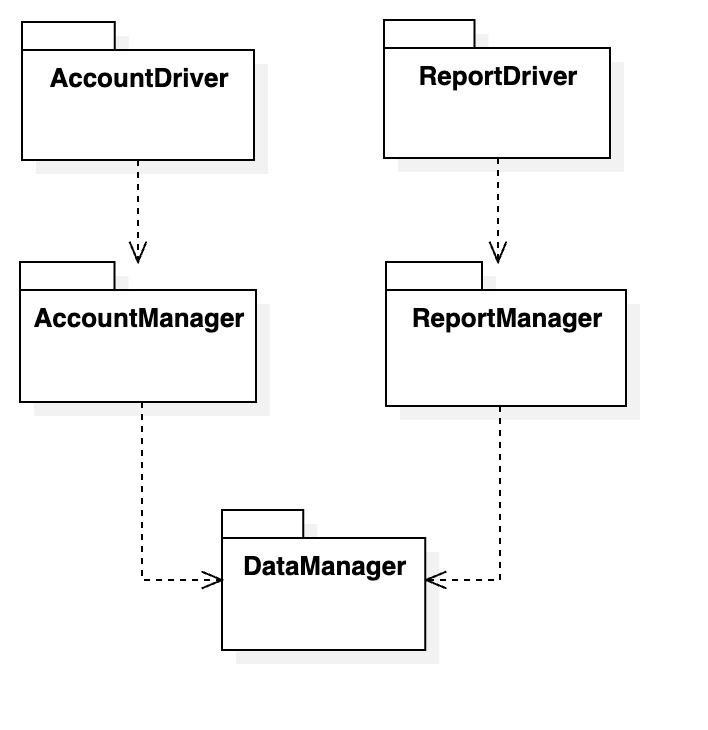
\includegraphics[width=0.6\linewidth]{DD//Images//Implementation/Stage2.jpg}
    \caption{Stage 2}
    \label{fig:placeholder}
\end{figure}

\newpage
\noindent
\textbf{Stage 3: Trip Orchestration Logic}
\vspace{2pt}

\noindent
In the third stage, we integrate the TripManager, which encompasses the NavigationManager and HistoryManager. The TripManager is integrated on top of the components validated in Stage 2. In particular, the integration tests focus on verifying the following interactions:

\begin{itemize}
    \item \textbf{Navigation Monitoring}: Verifying the core logic of the NavigationManager that, upon receiving real-time GPS updates, checks the user's adherence to the calculated path and computes real-time session statistics
    \item \textbf{User Statistics Update}: Verifying that the HistoryManager correctly invokes the ProfileManager (component of the AccountManager) exclusively upon trip completion to update the user’s aggregated statistics.
    \item \textbf{Report Submission}: Ensuring that the HistoryManager correctly forwards path data to the ReportManager when a trip is finalized.
    \item \textbf{Trip Persistence}: Verifying that the trip session data is correctly stored via the DataManager.
\end{itemize}

\noindent
A Trip Driver is used to simulate the full lifecycle of a trip (start, location updates, stop), ensuring that the manager correctly coordinates these diverse dependencies.

\begin{figure}[H]
    \centering
    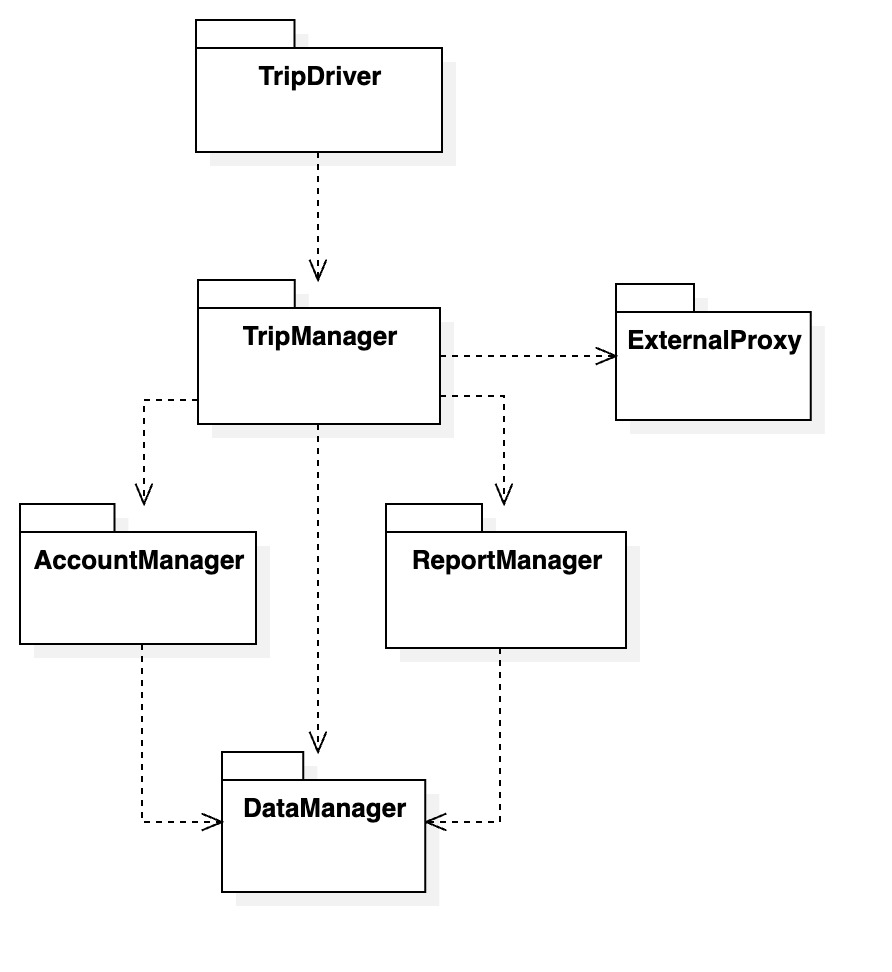
\includegraphics[width=0.6\linewidth]{DD//Images//Implementation/Stage3.jpg}
    \caption{Stage 3}
    \label{fig:placeholder}
\end{figure}

\newpage
\noindent
\textbf{Stage 4: Final Application Server Integration}
\vspace{2pt}

\noindent
The final stage completes the Application Server integration by adding the PathManager. This component is responsible for the core routing algorithms and relies on internal trip management subsystem. In this phase, we integrate the PathManager with the components validated in Stage 3. While covering the entire operational scope of the component, the integration process places particular emphasis on the following critical interactions:

\begin{itemize}
    \item \textbf{Automated mode trip Logic Integration}: Verifying that the PublishedPathManager can correctly access the TripManager (specifically the HistoryManager) to save the details of completed automated trip into the user's history.
    \item \textbf{Full System Flow}: Executing scenarios where the Path Driver triggers the complete operational chain: "Search Path (PathManager) -> Start Navigation (TripManager) -> Complete Trip -> Save to History \& Submit Report (TripManager) -> Update User Statistics (ProfileManager)". This verifies that the path object provided by the search logic is correctly interpreted by the navigation engine and that all side effects, persisting the trip history, submitting the report for merging, and updating user statistics are successfully committed.
\end{itemize}

\noindent
At the conclusion of this stage, the backend logic is fully integrated. The Test Drivers can then be replaced by the actual Web Server and Client Application for the System Testing phase.


\begin{figure}[H]
    \centering
    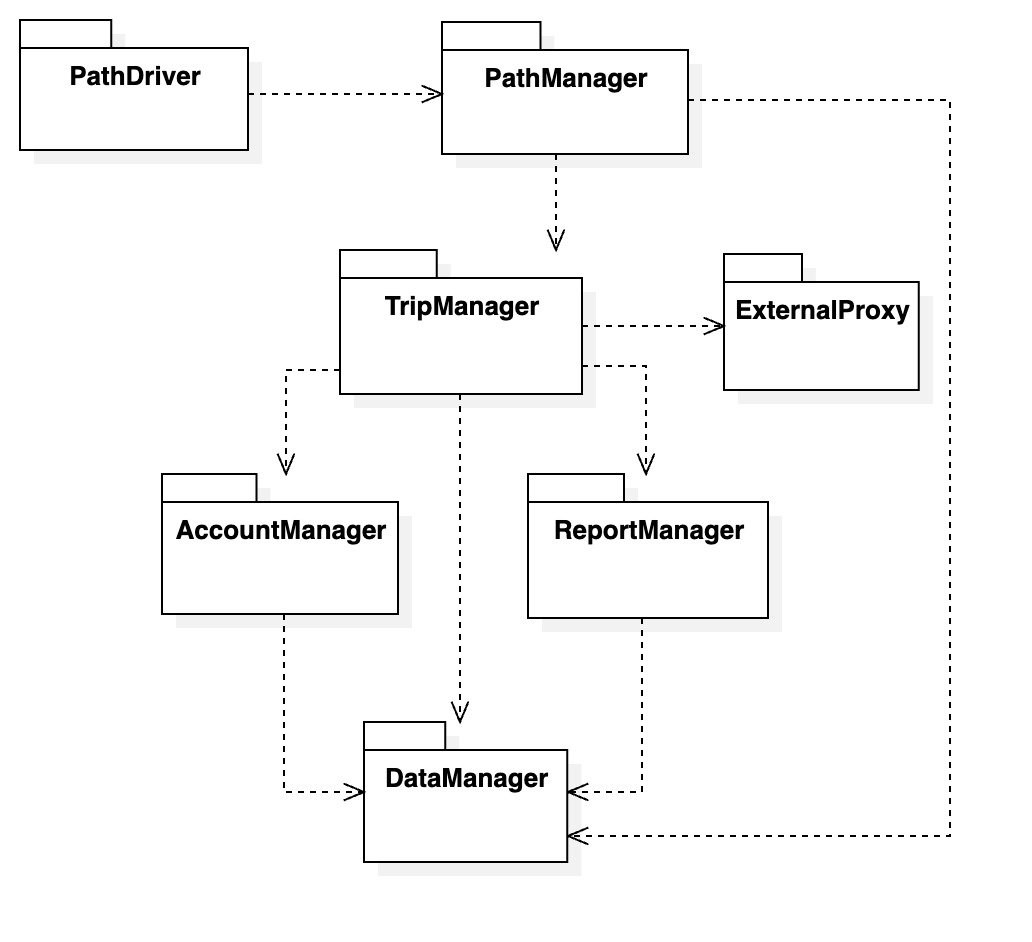
\includegraphics[width=0.6\linewidth]{DD//Images//Implementation/Stage4.jpg}
    \caption{Stage 4}
    \label{fig:placeholder}
\end{figure}

\newpage
\subsection{System Testing}
Once all the Application Server components have been integrated and the mock drivers replaced by the actual Web Server and Client interfaces, System Testing begins. This process aims at verifying both functional and non-functional requirements and must take place in a testing environment that mirrors the production configuration as closely as possible. Specifically, the system will be subjected to the following testing categories:

\begin{itemize}
    \item \textbf{Functional Testing}: It ensures that the requirements and specifications defined in the RASD are properly satisfied by the System. In this phase, we verify the complete end-to-end user flows.
    \item \textbf{Performance Testing}: The main purpose is to identify and eliminate performance bottlenecks affecting response time and throughput.
    \item \textbf{Load Testing}: It aims at detecting bugs such as memory leaks and buffer overflows, identifying the maximum operating capacity of the application.
    \item \textbf{Stress Testing}: It verifies the stability and reliability of the software application under extreme conditions. The goal is to ensure robustness and proper error handling.
    
\end{itemize}






